\newcommand{\U}[1]{\ensuremath{\,\textrm{#1}}}
\newcommand{\tref}{\ensuremath{\textrm{ref}}}
\newcommand{\vthref}{\ensuremath{v_\textrm{thref}}}


\documentclass[a4paper]{report}
\usepackage{fullpage}
\usepackage{amsmath}
\usepackage{amssymb}
\usepackage{bm}
\usepackage{graphicx}
\usepackage{tabularx}
\usepackage{hyperref}

\hypersetup{bookmarks, plainpages=false, colorlinks=true, pdfborder={0 0 0 0}, linkcolor=blue, citecolor=blue, urlcolor=blue, pdftitle={GKDB documentation}}
\newcolumntype{Y}{>{\centering\arraybackslash}X}
\newcolumntype{R}{>{\hsize=0.4\hsize}Y}
\newcolumntype{S}{>{\hsize=0.6\hsize}Y}
\newcolumntype{T}{>{\hsize=0.8\hsize}Y}
\newcolumntype{L}{>{\hsize=1.2\hsize}X}

\begin{document}

\title{Documentation of the  gyrokinetic database GKDB}

\author{Y. Camenen on behalf of the GKDB working group}

\date{Last update: January 8, 2018}

\maketitle


\tableofcontents

\chapter{Preamble}

This document summarises the names, conventions and normalisations adopted for the inputs and outputs of the linear gyrokinetic database (GKDB) storing results from $\delta$f, flux-tube gyrokinetic simulations.\\ 
The normalised inputs and outputs are independent of $\rho^*$ consistently with the local approximation and a spectral representation is assumed in the perpendicular plane (i.e. homogeneous turbulence).\\
S.I. units are used everywhere with the exception of temperatures given in eV. This means that $kT$ is noted $T$ as is customary in plasma physics (and possibly confusing).

\chapter{Conventions and normalisations}
\label{chap:normdef}
\section{Cylindrical and flux coordinate systems}
The ITER coordinate convention is adopted for the GKDB. The corresponding index in the COordinate COnventionS system  \cite{Sauter:CPC2013} is COCOS=$11$.
\subsection{Cylindrical coordinate system $(R,\varphi,Z)$}
A right-handed cylindrical coordinate system $(R,\varphi,Z)$, with $R$ the major radius, $Z$ the elevation and $\varphi$ the toroidal angle (increasing when anticlockwise from above) is used to describe the flux surfaces, see Fig.~\ref{fig:coord1}. \\
The magnetic equilibrium is assumed to be axisymmetric and the poloidal contours of the flux surface $\Psi(R,Z)=\Psi_0$, with $\Psi$ the poloidal magnetic flux, are noted $\{R_{\Psi_0},Z_{\Psi_0}\}$.

\begin{figure}[h]
\begin{center}
  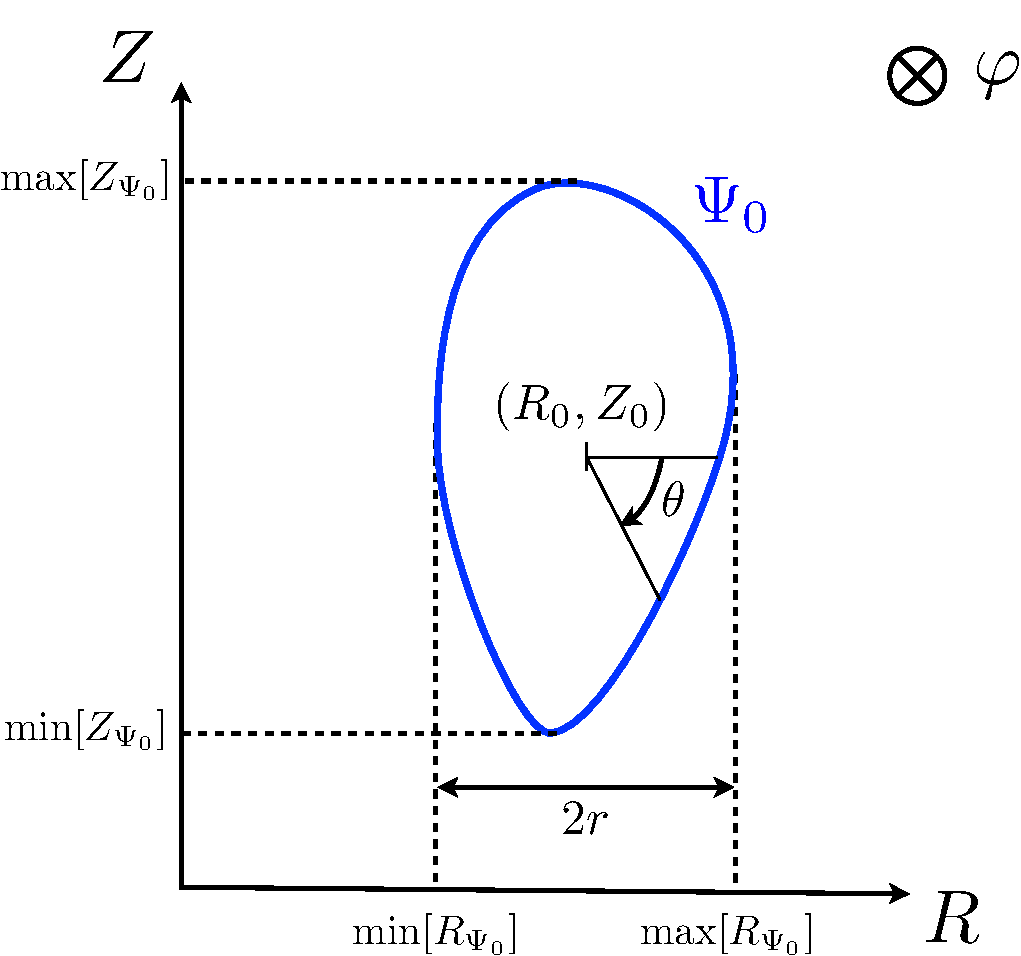
\includegraphics[width=9cm]{COCOS.pdf}\\
  \caption{\label{fig:coord1} Coordinate conventions used in the GKDB (COCOS=11, \cite{Sauter:CPC2013}).}
\end{center}
\end{figure}

\subsection{Flux coordinate system $(r,\theta,\varphi)$}
A right handed flux coordinate system $(r,\theta,\varphi)$ is now introduced.
\subsubsection{Flux surface center}
To start with, a reference point $(R_0,Z_0)$ is defined for the flux surface of interest $\{R_{\Psi_0},Z_{\Psi_0}\}$:
\begin{eqnarray}
 R_0 &=& \frac{1}{2}\left[\max[R_{\Psi_0}] + \min[R_{\Psi_0}]\right]\\
 Z_0 &=& \frac{1}{2}\left[\max[Z_{\Psi_0}] + \min[Z_{\Psi_0}]\right]
\end{eqnarray} 
The reference point  $(R_0,Z_0)$ will be used in the following to define the poloidal angle. Note that $(R_0,Z_0)$ is not the position of the magnetic axis, although it can be in some particular cases. 

\subsubsection{Radial coordinate}
The radial coordinate $r$ is defined as 
\begin{equation}
 r = \frac{1}{2}\left[\max[R_{\Psi_0}] - \min[R_{\Psi_0}]\right]
\end{equation}
It has the dimension of a length and is constant on a flux surface, by definition. The radial coordinate of the flux surface $\Psi=\Psi_0$ is noted $r_0$.

\subsubsection{Poloidal angle}
The poloidal angle is defined from the following relationships:
\begin{eqnarray}
 \cos \theta &=& \frac{R_{\Psi_0}-R_0}{\left[ (R_{\Psi_0}-R_0)^2 + (Z_{\Psi_0}-Z_0)^2 \right]^{1/2}}\\
 \sin \theta &=& -\frac{Z_{\Psi_0}-Z_0}{\left[ (R_{\Psi_0}-R_0)^2 + (Z_{\Psi_0}-Z_0)^2 \right]^{1/2}}
\end{eqnarray}
The poloidal angle is zero at the low field side midplane (the midplane is defined with respect to the flux surface $\Psi=\Psi_0$ and corresponds to $Z=Z_0$) and increases clockwise when the tokamak vertical axis is on the left of the flux surface, see Fig.~\ref{fig:coord1}.

\section{Flux surface average}
In a few cases, flux surface averaged quantities will be required. We adopt here the flux surface average definition that arises when taking the integral of a conservation equation over the volume enclosed by a flux surface (i.e. the standard procedure to built 1D transport equations in tokamaks, see for instance \cite{Hinton:RMP1976}).\\
The flux surface average of a quantity $A$ is then given by
\begin{equation}
 <A> = \frac{\int A(\mathbf{x}) \delta(r-r_0) \,\textrm{d}^3{x}}{\int\delta(r-r_0) \,\textrm{d}^3{x}}
\end{equation}
where $r_0$ is the radial coordinate of the flux surface on which the average is being 
performed, $r$ is the value of the radial coordinate at position $\mathbf{x}$, $\delta$ is the Dirac function and the integral is being performed over the whole plasma volume (or entire world, it does not matter).  \\
Noting that the surface element $\textrm{d} S$ on a flux surface is related to the volume element 
$\textrm{d}^3x$ by
\begin{equation}
 \textrm{d}^3x = \textrm{d} S \frac{\textrm{d}r}{|\nabla r|}
\end{equation}
with $r$ an arbitrary flux surface label (taken here to be the radial coordinate defined above), a convenient alternative (and equivalent) expression for the flux surface average is obtained:
\begin{equation} 
 <A> = \frac{1}{V'} \oint A \frac{\textrm{d}S}{|\nabla r|}
\end{equation}
with $V'= \frac{\partial V}{\partial r}$ and $V$ being the volume enclosed by the flux surface labelled by $r$. 

\section{Normalisations}
All quantities in the database (inputs and outputs) are normalised with respect to the reference quantities introduced in this section. Six reference quantities are first introduced (fundamental reference quantities) and then used to built other convenient normalising factors (derived reference quantities).\\
In principle, reference quantities do not need to be specified, as the purpose of the database is to relate normalised inputs to normalised outputs. 
However, if the choice of reference quantities is left arbitrary, the same physical inputs could lead to different normalised inputs in the database depending on the normalisation choice. This is not desirable and the reference quantities are therefore imposed. 

\subsection{Fundamental reference quantities}
The six fundamental reference quantities are:
\begin{itemize}
\item $q_\tref=e=1.6022\times10^{-19}\U{C}$, the positive elementary charge
\item $m_\tref=m_D=3.3445\times10^{-27}\U{kg}$, the Deuterium mass
\item $T_\tref=T_e(r_0,\theta=0)$, the electron temperature at $\theta=0$
\item $n_\tref=n_e(r_0,\theta=0)$, the electron density at $\theta=0$
\item $L_\tref=R_0$, the reference length
\item $B_\tref=B_t(R_0,Z_0)$, the reference magnetic field (toroidal magnetic field at the flux surface center)
\end{itemize}

\subsection{Derived reference quantities}
For convenience, the following reference quantities are defined:
\begin{itemize}
\item $\vthref=\sqrt{\frac{2T_\tref}{m_\tref}}$, the reference thermal velocity
\item $\rho_\tref = \frac{m_\tref \vthref}{q_\tref B_\tref}$, the reference Larmor radius
\end{itemize}


\chapter{Inputs}
\section{Species}
For each species $s$, the background distribution function is supposed to be a local Maxwellian. Poloidal asymmetry in the background induced by centrifugal effects is allowed. Poloidally asymmetric quantities are given in input at $\theta=0$. Poloidal asymmetry induced by anisotropic temperatures is not included yet, but could be introduced if need be.\\ 
At this stage, the database only stores runs with kinetic electron species (adiabatic electrons not allowed). An arbitrary number of kinetic species is allowed, but quasineutrality has to be ensured.

\subsection{Charge}
$$Z_{sN}=\frac{q_s}{q_\tref}$$
\subsection{Mass}
$$m_{sN}=\frac{m_s}{m_\tref}$$
\subsection{Density}
$$n_{sN}=\frac{n_s}{n_\tref}$$
\subsection{Logarithmic density gradient}
$$L_\tref/L_{n_s}=-L_\tref \frac{1}{n_s}\frac{\partial n_s}{\partial r}$$
Positive for peaked profiles. 
\subsection{Temperature}
$$T_{sN}=\frac{T_s}{T_\tref}$$
\subsection{Logarithmic temperature gradient}
$$L_\tref/L_{T_s}=-L_\tref \frac{1}{T_s}\frac{\partial T_s}{\partial r}$$
Positive for peaked profiles.
\subsection{Toroidal velocity}
$$u_{N}=\frac{L_\tref}{\vthref}\omega_{\Phi}$$
Positive for a flow in the direction of $\nabla \varphi$.\\
All species are assumed to have a purely toroidal flow $\mathbf{v}_s=R^2\omega_\Phi\nabla \varphi$ with a common toroidal angular frequency proportional to the background electric field:
$$\omega_{\Phi}=-s_j\frac{1}{|\nabla \Psi|}\frac{\partial \Phi}{\partial r},$$
with $\Phi$ the background electrostatic potential. This assumption is consistent with the ordering used in local gyrokinetic codes, as $\omega_\Phi$ is the lowest order flow in a $\rho_*$ expansion according to neoclassical theory \cite{Hirshman:NF1981}.

\subsection{Toroidal velocity gradient}
$$u'_{sN}=-\frac{L_\tref^2}{\vthref}\frac{\partial \omega_{\varphi,s}}{\partial r}$$
Positive for peaked profiles of a flow in the direction of $\nabla \varphi$.\\
Note that the possibility to have a species dependent toroidal velocity gradient with $\omega_{\varphi,s}\neq \omega_\Phi$ is retained. Strictly speaking, this is inconsistent with the local limit assumption $\rho_*\rightarrow 0$ but can be interesting for the interpretation of the experiments (see the discussion in section II of \cite{Camenen:PoP2016} for more details).


\subsection{Summary of the species parameters}
\begin{tabularx}{\textwidth}{|X|Y|Y|Y|}
\hline
Name & Value/Range & Type & Dimension \\
\hline
charge & - & Integer & $N_\textrm{species}$ \\
mass & $>0$ & Real & $N_\textrm{species}$ \\
density & $\geq0$ & Real & $N_\textrm{species}$  \\
density\_log\_gradient & - & Real & $N_\textrm{species}$\\
temperature & $>0$ & Real & $N_\textrm{species}$ \\
temperature\_log\_gradient & - & Real & $N_\textrm{species}$ \\
toroidal\_velocity & - & Real & 1 \\
toroidal\_velocity\_gradient & - & Real & $N_\textrm{species}$  \\
\hline
\end{tabularx}\\
All parameters above are species dependent, except the toroidal velocity that is common to all species. 

\section{Magnetic equilibrium}
The magnetic equilibrium in the vicinity of the flux surface of interest is specified by the parameters described in this section, given at $r=r_0$.

\subsection{Radial position}
$$r_N=\frac{r_0}{L_\tref}$$

%\subsection{Reference point}
%$$R_{0N} = \frac{R_0}{L_\tref} \qquad \textrm{and} \qquad Z_{0N}=\frac{Z_0}{L_\tref}$$

\subsection{Toroidal field direction}
$$s_b = \textrm{sign}[\mathbf{B}\cdot\nabla\varphi]$$

\subsection{Toroidal current direction}
$$s_j = \textrm{sign}[\mathbf{j}\cdot\nabla\varphi]$$
with $j$ the plasma current density. For the conventions adopted in this document, positive plasma current implies positive poloidal magnetic field.

\subsection{Safety factor}
$$q=\frac{1}{2\pi}\int_0^{2\pi} \frac{\mathbf{B}\cdot\nabla \varphi}{\mathbf{B}\cdot\nabla \theta}\,\textrm{d}\theta$$
Note that $q$ can be positive or negative, its sign depends on the sign of the toroidal plasma current and magnetic field:
$$q = s_b s_j |q|$$

\subsection{Magnetic shear}
$$\hat{s}=\frac{r}{q}\frac{\partial q}{\partial r}$$


\subsection{Pressure gradient}
$$p'_N = -\frac{2\mu_0 L_\tref}{B_\tref^2 }\frac{\partial p}{\partial r}$$
with $p$ the total plasma pressure (i.e. the pressure term entering the Grad-Shafranov equation). $p'_N$ (often called $\beta'$) is a quantity related to the magnetic equilibrium and does not need to be consistent with the gradients ($L_\tref/L_{n_s}$, $L_\tref/L_{T_s}$) specified for the kinetic species.\\
Note that the low $\beta'$ approximation for the curvature drift, i.e. the approximation
$$\mathbf{b}\times(\mathbf{b}\cdot\nabla\mathbf{b})=\frac{1}{2}\mathbf{b}\times\nabla r\frac{2\mu_0}{B^2}\frac{\partial p}{\partial r} + \frac{\mathbf{B}\times\nabla B}{B^2} \sim  \frac{\mathbf{B}\times\nabla B}{B^2}, $$
is not allowed in the database as it is inconsistent with the use of a finite pressure gradient ($p'_N$) for the equilibrium description. 


\subsection{Plasma shape}
A general description of local magnetic equilibria particularly convenient for gyrokinetic codes was introduced by J. Candy in \cite {Candy:PPCF2009}. It is used in the GKDB with a few minor modifications.
The plasma shape is described by specifying the distance of the constant poloidal flux contours to the reference point $(R_0,Z_0)$  normalised to $L_\tref$:
$$ a_N(r,\theta) = \frac{1}{L_\tref}\sqrt{\left[R_{\Psi_0}(r,\theta)-R_0\right]^2 + \left[Z_{\Psi_0}(r,\theta)-Z_0\right]^2} $$
To allow regressions in the database the flux surface contours are parametrised as 
$$ a_N(r,\theta) = \sum_{n=0}^{N_{sh}} c_n \cos(n\theta) + s_n \sin(n\theta) $$
The specification of the local magnetic equilibrium then requires $4N_{sh}+2$ terms, given at $r=r_0$, where $N_{sh}$ is the degree of the expansion: $\{c_n,s_n,\frac{\partial c_n}{\partial r_N},\frac{\partial s_n}{\partial r_N}\}$. Typically $N_{sh}\leq8$ is sufficient to capture most of the plasma shapes but higher values can be used when needed.

\subsection{Summary of the shape parameters}
\begin{tabularx}{\textwidth}{|X|Y|Y|Y|}
\hline
Name & Value/Range & Type & Dimension \\
\hline
r\_minor & $0\leq r_N \leq 1$ & Real & 1 \\
ip\_sign & $\pm 1$ & Integer & 1 \\
b\_field\_tor\_sign & $\pm 1$ & Integer & 1 \\
q & - & Real & 1 \\
magnetic\_shear & - & Real & 1 \\
pressure\_gradient & - & Real & 1 \\
c & $\geq 0$ & Real & $N_{sh}+1$ \\
dc\_dr\_minor & - & Real & $N_{sh}+1$ \\
s & $\geq 0$ & Real & $N_{sh}$ \\
ds\_dr\_minor & - & Real & $N_{sh}$ \\
\hline
\end{tabularx}

\section{Modes}
As almost every gyrokinetic codes use a different coordinate system, it is convenient to specify the Fourier modes in a coordinate free form.\\
To define this coordinate free form, let's first call, $x$ and $y$, the radial and binormal coordinates used in gyrokinetic codes to describe the turbulence in the plane perpendicular to the magnetic field. The radial coordinate $x$ is assumed to be a flux label (i.e. $\mathbf{B}\cdot \nabla x =0$).
In a spectral representation, perturbed quantities are then written:
\begin{equation}
 f(x,y,\theta) = \sum_{k_x,k_y} \hat{f}(k_x,k_y,\theta)\exp[ik_x x + ik_y y] 
\end{equation}
where $\theta$ is used as the parallel coordinate.
For a given mode, the perpendicular wave vector (in real space) is given by:
\begin{equation}
 k_\perp^2(\theta) = k_x^2 g^{xx} + 2k_xk_y g^{xy} + k_y^2g^{yy}
\end{equation}
with the code dependent metric elements given by $g^{ij}=\nabla i \cdot \nabla j$. All the metric information is on the right hand side of the equation above, the resulting $k_\perp$ does not depend on the specific coordinate choices made in gyrokinetic codes.

\subsection{Radial wavevector}
The normalised coordinate independent radial wavevector is defined as
\begin{equation}
 k_{r*}\rho_\tref = k_x \sqrt{g^{xx}(\theta=0)} \rho_\tref
\end{equation}

\subsection{Binormal wavevector}
The normalised coordinate independent binormal wavevector is defined as
\begin{equation}
 k_{\theta*}\rho_\tref = k_y \sqrt{g^{yy}(\theta=0)} \rho_\tref
\end{equation}

An alternative convenient specification of the binormal wavevector is the effective poloidal mode number normalised to the ion Larmor radius  $nq\rho_\tref/r_0$  \cite{Merlo:PoP2016}. This definition is also coordinate independent and related to a physical quantity. It will not be used here as there is no simple equivalent to specify the radial wave vector.

\section{Number of poloidal turns}
In the spectral representation of a flux-tube domain, the periodicity of the torus in the poloidal direction leads to the coupling of radial modes in the parallel direction:
$$\hat{f}(k_x,k_y,\theta-\pi)=\hat{f}(k_x+\Delta k_x,k_y,\theta+\pi)$$
with $\Delta k_x$ depending on the magnetic shear.\\
A flux-tube extending over an odd number $N_p$ of poloidal turns with 1 radial mode $k_x$ is therefore equivalent to a flux-tube extending over 1 poloidal turn with $N_p$ coupled radial modes $k_x + p\Delta k_x$ with $p$ an integer varying from $-(N_p-1)/2$ to $(N_p+1)/2$.\\ 
In practice, running with a sufficiently high number of poloidal turns (or coupled radial modes) is necessary to get a result independent of the boundary condition imposed at the end of the field line (when the number of poloidal turns increases, $k_\perp$ increases and the perturbations are damped by finite Larmor radius effects). 

\subsection{Summary of the mode parameters}
\begin{tabularx}{\textwidth}{|X|Y|Y|Y|}
\hline
Name & Value/Range & Type & Dimension \\
\hline
radial\_wavevector & - & Real & 1 \\
binormal\_wavevector & $\geq 0$ & Real & 1 \\
poloidal\_turns & $>0$ & Integer & 1 \\
\hline
\end{tabularx}

\section{Electromagnetic effects}
\subsection{Plasma beta}
The strength of the electromagnetic effects depends on the ratio of the plasma pressure to the magnetic energy and is specified by the dimensionless ratio:
\begin{equation}
\beta_{eN} = 2\mu_0 \frac{n_\tref T_\tref}{B_\tref^2}
\end{equation}
The plasma beta entering the Amp\`ere's law is obtained from the reference value above combined with the species parameters (normalised density and temperature).
When $\beta_{eN}=0$, the run is electrostatic. 

\subsection{Switches}
\begin{itemize}
\item Are the fluctuations of the parallel electromagnetic vector potential $A_\parallel$ retained (magnetic field flutter)?
\item Are the fluctuations of the perpendicular electromagnetic vector potential retained (magnetic field compression)?
\end{itemize}

\subsection{Summary of the electromagnetic effects parameters}
\begin{tabularx}{\textwidth}{|X|Y|Y|Y|}
\hline
Name & Value/Range & Type & Dimension \\
\hline
beta & $\geq 0$ & Real & 1 \\
include\_a\_parallel & 0 or 1 & Logical & 1 \\
include\_b\_field\_parallel & 0 or 1 & Logical & 1 \\
\hline
\end{tabularx}

\section{Collisions and Debye length}
\subsection{Plasma collisionality}
The normalised collision frequency
\begin{equation}
 \nu_{eN} = \frac{q_\tref^4}{4\pi\epsilon_0^2}\frac{R_\tref n_\tref}{T_\tref^2}
\end{equation}
is used to specify the plasmas collisionality, with $R_\tref$ in $[\textrm{m}]$, $n_\tref$ in $[\textrm{m}^{-3}]$ and $T_\tref$ in $[\textrm{eV}]$. It is assumed that each species collisionality is calculated in the code consistently with the species input parameters (i.e. the normalised species temperature and density are used to calculate the collisionality of each species). This behaviour can be altered by specific collisionality switches described in Sec.~\ref{sec:colswitches}.\\

\subsection{Collisionality related switches} \label{sec:colswitches}
\begin{itemize}
\item Pitch angle scattering only is retained (as opposed to pitch angle and energy scattering)
\item Electron-ion collisions only are retained (as opposed to all interspecies collisions)
\item Enhancement factor for electron to (main) ion collisions. This is typically used to mimic the impact of impuritites on the electron-ions collisions. The enhancement factor multiplies the electron to main ion collisionality.
\item Is momentum conservation ensured?
\item Is energy conservation ensured?
\item Are finite Larmor radius effects retained in the collision treatment?
\end{itemize}
Note that the implementation of collisions is highly code dependent and the list above does not give a complete characterisation of how collisions were treated in the run. However, this information can be retrieved from the specific code input file used for the run, which is also stored in the database, and the code documentation,\\

\subsection{Debye length}
The Debye length
\begin{equation}
 \lambda_{D}= \sqrt{\frac{\epsilon_0 T_\tref}{n_\tref q_\tref^2}}
\end{equation}
enters the linearized quasi-neutrality equation. When neglected, this term is set to zero.

\subsection{Summary of the collision parameters}
\begin{tabularx}{\textwidth}{|L|S|S|S|}
\hline
Name & Value/Range & Type & Dimension \\
\hline
collisionality & $\geq 0$ & Real & 1 \\
collision\_enhancement\_factor & $\geq 1$ & Real & 1 \\
collision\_pitch\_only & 0 or 1 & Logical & 1 \\
collision\_ei\_only & 0 or 1 & Logical & 1 \\
collision\_momentum\_conservation\_flag & 0 or 1 & Logical & 1 \\
collision\_energy\_conservation\_flag & 0 or 1 & Logical & 1 \\
collision\_finite\_larmor\_radius & 0 or 1 & Logical & 1 \\
debye\_length & $\geq 0$ & Real & 1 \\
\hline
\end{tabularx}


\section{Various switches} \label{sec:rotswitches}
\begin{itemize}
\item Are the centrifugal effects included?  
\item Was it an initial value or eigenvalue run?
\end{itemize}

\subsection{Summary of the other switches}
\begin{tabularx}{\textwidth}{|X|Y|Y|Y|}
\hline
Name & Value/Range & Type & Dimension \\
\hline
include\_centrifugal\_effects &  0 or 1 & Logical & 1 \\
initial\_value\_run &  0 or 1 & Logical & 1 \\
\hline
\end{tabularx}

\section{Meta-data}

\subsection{Code input file}
The code input files are automatically parsed and all the code specific inputs stored in a large key/value table. They can be retrieved if/when needed.

\subsection{Meta-data}
For each point in the database, the following information is requested 
\begin{itemize}
 \item The name of the code 
 \item The version of the code
 \item The name of the person submiting the entry to the database
\end{itemize}

\subsection{Comments and tags}
Informative comments can also be added. For instance to indicate whether this entry is based on an experimental case or if it was used in a publication.\\
Different entries can be grouped together by giving them a common tag. This can be interesting when submitting entries from a parameter scan.
 
\subsection{Summary of the meta-data}
\begin{tabularx}{\textwidth}{|X|Y|Y|Y|}
\hline
Name & Value/Range & Type & Dimension \\
\hline
name &  - & String & 1 \\
version &  - & String & 1 \\
creator &  - & String & 1 \\
comment &  - & String & 1 \\
tag  &  - & String & $N_\textrm{tags}$ \\
\hline
\end{tabularx}


\chapter{Outputs}
\section{Mode amplitude}
In linear runs, unstable modes are exponentially growing in time and so are the associated fluxes. 
The exponentially growing outputs stored in the database are therefore normalised to a dimensionless mode amplitude defined as:
\begin{equation}
 A_f(k_x,k_y) = \sqrt{\frac{1}{2\pi}\left.\int \left[|\hat{\phi}_N(k_x,k_y,\theta)|^2 + |\hat{A}_{\parallel N}(k_x,k_y,\theta)|^2  + |\hat{B}_{\parallel N}(k_x,k_y,\theta)|^2\right] \,\textrm{d}\theta \right.}
\end{equation}
with the Fourier components of the electrostatic potential and vector potential normalised as follows:
\begin{equation}
  \hat{\phi}_N = \frac{1}{\rho_*}\frac{q_\tref}{T_\tref} \hat{\phi} \qquad \qquad 
  \hat{A}_{\parallel N}=\frac{1}{\rho_*^2}\frac{1}{L_\tref B_\tref} \hat{A}_\parallel \qquad \qquad
  \hat{B}_{\parallel N}=\frac{1}{\rho_*}\frac{1}{B_\tref} \hat{B}_\parallel
\end{equation}
where $\rho_*=\rho_\tref/L_\tref$. The integral over $\theta$ is performed over the full length of the flux-tube (it is equivalent to an integral over one poloidal turn of the sum of all connected $k_x$ modes).\\
The value of the mode amplitude in a linear run has little meaning by itself and is not stored in the database. 

\section{Mode growth rate and frequency}
The normalisations of the mode growth rate $\gamma$ and frequency $\omega_r$ are:
\begin{equation}
 \gamma_N(k_x,k_y) = \gamma(k_x,k_y) \frac{L_\tref}{v_\textrm{thref}} \qquad \qquad \textrm{and} \qquad \qquad \omega_{rN}(k_x,k_y) = \omega_r(k_x,k_y) \frac{L_\tref}{v_\textrm{thref}}
\end{equation}
By convention, unstable modes have a positive growth rate and modes propagating in the ion diamagnetic drift direction have a positive frequency (and therefore a negative frequency when they are propagating in the electron diamagnetic drift direction).\\

For initial value runs, the following (post-processing) method is used to determine the tolerance on the run convergence:
$$\gamma_\textrm{tol} = \frac{1}{\gamma_f}\sqrt{\frac{1}{\Delta t}\int_{t_f-\Delta t}^{t_f} \left[\gamma(t)-\gamma_f\right]^2\,\textrm{dt}}$$
where $t_f$ and $\gamma_f$ are the time and growth rate at the end of the simulation, respectively, $\Delta t = 3/\gamma_f$ and
$$\gamma(t)=\frac{1}{\delta t}[\ln{A_f(t)}-\ln{A_f(t-\delta t)}]$$
with $\delta t$ depending on the code setup but in any case several times smaller than $\Delta t$. Note that any exponentially growing quantity can be used in place of $A_f$ to compute the time dependent growth rate.

\subsection{Summary of the eigenvalue outputs}
\begin{tabularx}{\textwidth}{|X|Y|Y|Y|}
\hline
Name & Value/Range & Type & Dimension \\
\hline
growth\_rate & - & Real & $N_\textrm{modes}$ \\
growth\_rate\_tolerance & $0<\gamma_\textrm{tol}\leq 0.1$ & Real & 1 \\
frequency & - & Real & $N_\textrm{modes}$ \\
\hline
\end{tabularx}
For initial value runs, $N_\textrm{modes}=1$ and only the linear outputs corresponding to the most unstable run are given. When the eigenvalue solver is used $N_\textrm{modes}$ indicates the number of modes for which the linear outputs are given. The tolerance on the growth rate still needs to be defined when an eigenvalue solver is used (input welcome!).




\section{Gyro-center fluxes}
\subsection{Definition}
For each species, the flux-surface averaged contravariant radial component of the particle flux, energy flux and toroidal angular momentum flux are given by:
\begin{eqnarray}
 \Gamma_s &=& \left<\int f_s \left[\mathbf{v}_\mathbf{E} + \mathbf{v}_{\mathbf{B}_\perp} + \mathbf{v}_{\nabla B_\parallel}  \right]\cdot \nabla r\,\textrm{d}\mathbf{v}\right> \\
  \Pi_s   &=& \left<\int s_b m_s R \frac{B_t}{B}v_\parallel f_s  \left[\mathbf{v}_\mathbf{E} + \mathbf{v}_{\mathbf{B}_\perp} + \mathbf{v}_{\nabla B_\parallel}  \right] \cdot \nabla r\,\textrm{d}\mathbf{v}\right> \\
      Q_s &=& \left<\int \frac{1}{2}m_sv^2 f_s \left[\mathbf{v}_\mathbf{E} + \mathbf{v}_{\mathbf{B}_\perp} + \mathbf{v}_{\nabla B_\parallel}  \right] \cdot \nabla r\,\textrm{d}\mathbf{v}\right> 
\end{eqnarray}
where $f_s$ is the perturbed guiding center distribution function of species $s$ and the two terms on the right hand side correspond to the fluxes induced by the electrostatic, magnetic flutter and magnetic compression drifts:
\begin{equation}
 \mathbf{v}_\mathbf{E} = \frac{\mathbf{b}\times \nabla \left<\phi\right>_\textrm{gy} }{B} \qquad \qquad \qquad
 \mathbf{v}_{\mathbf{B}_\perp} = -v_\parallel \frac{\mathbf{b}\times \nabla \left<A_{\parallel}\right>_\textrm{gy}}{B}  \qquad \qquad \qquad
 \mathbf{v}_{\nabla B_\parallel} = \frac{\mu}{Ze} \frac{\mathbf{b}\times \nabla \left<B_{\parallel}\right>_\textrm{gy}}{B}
\end{equation}
with $\left<\phi\right>_\textrm{gy}$, $\left<A_{\parallel}\right>_\textrm{gy}$ and $\left<B_{\parallel}\right>_\textrm{gy}$, the gyro-averaged perturbed electrostatic potential, parallel vector potential and parallel magnetic field, respectively. The fluxes are positive when outward (for a transported quantity that is positive).\\
Note that the momentum flux in the expression above only includes the toroidal projection of the parallel momentum. The toroidal projection of the perpendicular momentum also contributes to the total momentum flux, see e.g. \cite{Scott:PoP2010}. This contribution is not included here but could be added in the future. 

\subsection{Laboratory frame versus rotating frame}
To describe inertial effects associated with the background rotation, several gyrokinetic codes (e.g. GKW, GENE, GS2) solve the gyro-kinetic equation in the frame rotating as a rigid body with the angular frequency $\omega_\Phi$. The Laboratory frame fluxes are of course the relevant ones for comparison with the experiments. They are related to quantities expressed in the rotating frame as follows:
\begin{eqnarray}
\Gamma_s^\textrm{L} &=& \Gamma_s^\textrm{co} \\
\Pi_s^\textrm{L} &=& \Pi_s^\textrm{co} + \left< \int m_s\omega_\Phi\left(\frac{RB_t}{B}\right)^2 f_s \mathbf{v}_\chi\cdot \nabla r  \,\textrm{d}\mathbf{v}\right>\\
Q_s^\textrm{L} &=& Q_s^\textrm{co} + \omega_\Phi \Pi_s^\textrm{co}
+ \left< \int \frac{1}{2}m_s(R\omega_\Phi)^2 f_s  \mathbf{v}_\chi\cdot \nabla r \,\textrm{d}\mathbf{v}\right> 
%Q_s^\textrm{L} &=& Q_s^\textrm{co} + \left< \int m_sv_\parallel\omega_\Phi\frac{RB_t}{B} f_s \mathbf{v}_\chi\cdot \nabla r  \,\textrm{d}\mathbf{v}\right> 
%+ \left< \int \frac{1}{2}m_s(R\omega_\Phi)^2 f_s  \mathbf{v}_\chi\cdot \nabla r \,\textrm{d}\mathbf{v}\right> 
\end{eqnarray}
with $\mathbf{v}_\chi=\mathbf{v}_\mathbf{E} + \mathbf{v}_{\mathbf{B}_\perp}+ \mathbf{v}_{\nabla B_\parallel}$ and all the expressions in the right hand sides evaluated in the rotating frame.
For convenience, both the Laboratory frame and rotating frame fluxes are stored in the database. 


\subsection{Normalisation}
The fluxes are given for each Fourier mode, normalised to the corresponding (linear) mode amplitude and made dimensionless as follows:
\begin{eqnarray}
 \Gamma_{Ns}(k_x,k_y) &=& \frac{1}{A_f^2}\frac{\Gamma_s(k_x,k_y)}{n_\tref \vthref \rho_*^2}\\
 \Pi_{Ns}(k_x,k_y) &=& \frac{1}{A_f^2}\frac{\Pi_s(k_x,k_y)}{n_\tref m_\tref L_\tref \vthref^2 \rho_*^2}\\
 Q_{Ns}(k_x,k_y) &=& \frac{1}{A_f^2}\frac{Q_s(k_x,k_y)}{n_\tref T_\tref \vthref \rho_*^2}
\end{eqnarray}
In addition, the electrostatic magnetic flutter and magnetic compressions are stored separately (e.g. $\Gamma_{Ns}=\Gamma_{Ns,\phi}+\Gamma_{Ns,A_\parallel}+\Gamma_{Ns,B_\parallel}$) for each flux. Note that the $\rho_*^2$ factor is included in $A_f^2$.

\subsection{Summary of the fluxes outputs}
\begin{tabularx}{\textwidth}{|L|S|S|S|}
\hline
Name & Value/Range & Type & Dimension \\
\hline
particle\_phi\_potential\_lab\_frame & - & Real & $N_\textrm{species}\times N_\textrm{modes}$\\ 
particle\_a\_parallel\_lab\_frame & - & Real & $N_\textrm{species}\times N_\textrm{modes}$\\ 
particle\_b\_field\_parallel\_lab\_frame & - & Real & $N_\textrm{species}\times N_\textrm{modes}$\\ 
momentum\_phi\_potential\_lab\_frame & - & Real & $N_\textrm{species}\times N_\textrm{modes}$\\ 
momentum\_a\_parallel\_lab\_frame & - & Real & $N_\textrm{species}\times N_\textrm{modes}$\\ 
momentum\_b\_field\_parallel\_lab\_frame & - & Real & $N_\textrm{species}\times N_\textrm{modes}$\\ 
heat\_phi\_potential\_lab\_frame & - & Real & $N_\textrm{species}\times N_\textrm{modes}$\\ 
heat\_a\_parallel\_lab\_frame & - & Real & $N_\textrm{species}\times N_\textrm{modes}$\\ 
heat\_b\_field\_parallel\_lab\_frame & - & Real & $N_\textrm{species}\times N_\textrm{modes}$\\ 
momentum\_phi\_potential\_co\_frame & - & Real & $N_\textrm{species}\times N_\textrm{modes}$\\ 
momentum\_a\_parallel\_co\_frame & - & Real & $N_\textrm{species}\times N_\textrm{modes}$\\ 
momentum\_b\_field\_parallel\_co\_frame & - & Real & $N_\textrm{species}\times N_\textrm{modes}$\\ 
heat\_phi\_potential\_co\_frame & - & Real & $N_\textrm{species}\times N_\textrm{modes}$\\ 
heat\_a\_parallel\_co\_frame & - & Real & $N_\textrm{species}\times N_\textrm{modes}$\\ 
heat\_b\_field\_parallel\_co\_frame & - & Real & $N_\textrm{species}\times N_\textrm{modes}$\\ 
\hline
\end{tabularx}

\section{Parallel mode structure}
\subsection{Parallel grid}
The variation of the mode amplitude and phase in the parallel direction is given as a function of the poloidal angle $\theta$ defined previously. Note that the poloidal angle grid does not need to be uniform.
\subsection{Perturbed electrostatic potential}
$$\phi_{Nf}(\theta) = \frac{\hat{\phi}_N(k_x,k_y,\theta)}{A_f(k_x,k_y)}\textrm{e}^{i\alpha}$$
The phase factor $\alpha$ is chosen so that the imaginary part of $\phi_{Nf}$ is zero at $\theta=0$ which makes comparisons of the mode structure between different runs easier.
When $|\phi_{Nf}(\theta=0)|=0$, $\alpha$ is taken to be zero.
 
\subsection{Perturbed parallel vector potential (magnetic field flutter)}
$$A_{\parallel Nf}(\theta) = \frac{\hat{A}_{\parallel N}(k_x,k_y,\theta)}{A_f(k_x,k_y)}\textrm{e}^{i\alpha}$$
\subsection{Perturbed parallel magnetic field (magnetic field compression)}
$$B_{\parallel Nf}(\theta) = \frac{\hat{B}_{\parallel N}(k_x,k_y,\theta)}{A_f(k_x,k_y)}\textrm{e}^{i\alpha}$$

\subsection{Moments of the distribution function}
Moments of the distribution function, expressed in the rotating frame, can also be stored in the database. The moments are given as a function of the poloidal angle $\theta$ for each species and Fourier mode and defined as follows:
\begin{align*}
\delta n_s(\theta,k_x,k_y) & =  \int \hat{f}_s(\theta,k_x,k_y) \,\textrm{d}\mathbf{v}& \delta n_s^{J_0}(\theta,k_x,k_y) & =  \int J_0(k_\perp\rho_s) \hat{f}_s(\theta,k_x,k_y) \,\textrm{d}\mathbf{v} \\
\delta v_{\parallel s}(\theta,k_x,k_y) & =  \int v_\parallel \hat{f}_s(\theta,k_x,k_y) \,\textrm{d}\mathbf{v}& \delta v_{\parallel s}^{J_0}(\theta,k_x,k_y) & =  \int v_\parallel J_0(k_\perp\rho_s) \hat{f}_s(\theta,k_x,k_y) \,\textrm{d}\mathbf{v}\\
\delta T_{\perp s}(\theta,k_x,k_y) & =  \int \frac{1}{2}m_s v_\perp^2 \hat{f}_s(\theta,k_x,k_y) \,\textrm{d}\mathbf{v}& \delta T_{\perp s}^{J_0}(\theta,k_x,k_y) & =  \int \frac{1}{2}m_s v_\perp^2 J_0(k_\perp\rho_s) \hat{f}_s(\theta,k_x,k_y) \,\textrm{d}\mathbf{v}\\
\delta T_{\parallel s}(\theta,k_x,k_y) & =  \int \frac{1}{2}m_s v_\parallel^2 \hat{f}_s(\theta,k_x,k_y) \,\textrm{d}\mathbf{v}& \delta T_{\parallel s}^{J_0}(\theta,k_x,k_y) & =  \int \frac{1}{2}m_s v_\parallel^2 J_0(k_\perp\rho_s) \hat{f}_s(\theta,k_x,k_y) \,\textrm{d}\mathbf{v}
\end{align*}
with $J_0$ the Bessel function. The normalisation of the moments is given by:
\begin{align*}
\delta n_{sN} & = \frac{\delta n_s}{n_\tref A_f\rho_*}& \delta n_{sN}^{J_0} & = \frac{\delta n_s^{J_0}}{n_\tref A_f\rho_*} \\
\delta v_{\parallel sN} & = \frac{\delta v_{\parallel s}}{\vthref A_f\rho_*}& \delta v_{\parallel sN}^{J_0} & = \frac{\delta v_{\parallel s}^{J_0}}{\vthref A_f\rho_*} \\
\delta T_{\perp sN} & = \frac{\delta T_{\perp s}}{n_\tref T_\tref A_f\rho_*}& \delta T_{\perp sN}^{J_0} & = \frac{\delta T_{\perp s}^{J_0}}{n_\tref T_\tref A_f\rho_*} \\
\delta T_{\parallel sN} & = \frac{\delta T_{\parallel s}}{n_\tref T_\tref A_f\rho_*}& \delta T_{\parallel sN}^{J_0} & = \frac{\delta T_{\parallel s}^{J_0}}{n_\tref T_\tref A_f\rho_*} 
\end{align*}


\subsection{Summary of the parallel outputs}
\begin{tabularx}{\textwidth}{|L|R|R|Y|}
\hline
Name & Value/Range & Type & Dimension \\
\hline
poloidal\_angle & $[-N_p\pi,N_p\pi]$ & Real & $N_\textrm{pol grid}$\\
phi\_potential\_perturbed & - & Complex & $N_\textrm{pol grid}\times N_\textrm{modes}$\\
a\_parallel\_perturbed & - & Complex & $N_\textrm{pol grid}\times N_\textrm{modes}$\\
b\_field\_parallel\_perturbed & - & Complex & $N_\textrm{pol grid}\times N_\textrm{modes}$\\ 
density\_moment & - & Complex & $N_\textrm{species}\times N_\textrm{pol grid}\times N_\textrm{modes}$\\
parallel\_velocity\_moment & - & Complex & $N_\textrm{species}\times N_\textrm{pol grid}\times N_\textrm{modes}$\\
parallel\_temperature\_moment & - & Complex & $N_\textrm{species}\times N_\textrm{pol grid}\times N_\textrm{modes}$\\
perpendicular\_temperature\_moment & - & Complex & $N_\textrm{species}\times N_\textrm{pol grid}\times N_\textrm{modes}$\\
J0\_density\_moment & - & Complex & $N_\textrm{species}\times N_\textrm{pol grid}\times N_\textrm{modes}$\\
J0\_parallel\_velocity\_moment & - & Complex & $N_\textrm{species}\times N_\textrm{pol grid}\times N_\textrm{modes}$\\
J0\_parallel\_temperature\_moment & - & Complex & $N_\textrm{species}\times N_\textrm{pol grid}\times N_\textrm{modes}$\\
J0\_perpendicular\_temperature\_moment & - & Complex & $N_\textrm{species}\times N_\textrm{pol grid}\times N_\textrm{modes}$\\
\hline
\end{tabularx}

\chapter{Derived quantities}
The derived quantities are computed internally when an entry is submitted to the GKDB and stored in the database. They can then be used for queries. 

\section{Relative fields amplitude}
The ratio of each field to the total mode amplitude is stored:
\begin{equation*}
A_\phi = \sqrt{\int |\phi_{Nf}(\theta)|^2\,\textrm{d}\theta}, \qquad \qquad
A_{A_\parallel} = \sqrt{\int |A_{\parallel Nf}(\theta)|^2\,\textrm{d}\theta}, \qquad \qquad
A_{B_\parallel} = \sqrt{\int |B_{\parallel Nf}(\theta)|^2\,\textrm{d}\theta}, 
\end{equation*}

\section{Fields parity}
The field parity with respect to $\theta=0$ is computed as follows:
\begin{equation*}
\pi_\phi = \frac{\left| \int \phi_{Nf}(\theta) \,\textrm{d}\theta \right|}{\int |\phi_{Nf}(\theta)| \,\textrm{d}\theta}, \qquad \qquad 
\pi_{A_\parallel} = \frac{\left| \int A_{\parallel Nf}(\theta) \,\textrm{d}\theta \right|}{\int |A_{\parallel Nf}(\theta)| \,\textrm{d}\theta}, \qquad \qquad 
\pi_{B_\parallel} = \frac{\left| \int B_{\parallel Nf}(\theta) \,\textrm{d}\theta \right|}{\int |B_{\parallel Nf}(\theta)| \,\textrm{d}\theta}
\end{equation*}

\section{Simplified shape description}
The flux surface elongation $\kappa$, top triangularity $\delta_\textrm{top}$ and bottom triangularity $\delta_\textrm{bot}$ are computed as follows:
\begin{equation*}
\kappa = \frac{Z_\textrm{max}-Z_\textrm{min}}{R_\textrm{max}-R_\textrm{min}}, \qquad \qquad \delta^\textrm{top} = \frac{R_{\Psi_0}(Z_\textrm{max})-R_0}{r_0}, \qquad \qquad \delta^\textrm{bot} = \frac{R_{\Psi_0}(Z_\textrm{min})-R_0}{r_0}
\end{equation*}
with $R_\textrm{min}=\min[R_{\Psi_0}]$, $R_\textrm{max}=\max[R_{\Psi_0}]$, $Z_\textrm{min}=\min[Z_{\Psi_0}]$ and $Z_\textrm{max}=\max[Z_{\Psi_0}]$.

\section{Global species parameters}
\subsection{Effective charge}
To have a fast and simple way to query on the plasma composition, the effective charge is computed:
$$Z_\textrm{eff} = \sum_\textrm{ions} n_{sN}Z_{sN}^2$$ 

\subsection{Sum over duplicated species}
To make query on entries with duplicate species more convenient, a duplicate species index is built that allow to query directly on:
$$n_{sN}=\sum_{s_i}n_{s_iN}, \qquad \qquad \frac{L_\tref}{L_{n_s}}=\frac{1}{n_{sN}}\sum_{s_i}n_{s_iN}\frac{L_\tref}{L_{n_{s_i}}}, \qquad \qquad \frac{L_\tref}{L_{T_s}}=\frac{1}{n_{sN}}\sum_{s_i}n_{s_iN}\frac{L_\tref}{L_{T_{s_i}}}$$
with $s_i$ the duplicated species entries for species $s$, identified by their common charge, mass and temperature.


\chapter{Entry submission procedure}
\section{Reference cases}

\section{Checks}
\subsection{Requirements}
\begin{itemize}
\item A species is identified by its charge, mass and temperature. The species with a negative charge is the electron species.
\item The charge, mass, temperature and density of the electron species are:
\begin{equation}
 Z_{eN}=-1, \qquad \qquad m_{sN} = 2.7237\times 10^{-4} \qquad \qquad T_{eN}=1 \qquad \qquad n_{eN}=1
\end{equation}
\item The species density and their gradients must satisfy quasineutrality:
\begin{equation}
 \sum_s Z_{sN}n_{sN} = 0 \qquad \qquad \sum_s Z_{sN}\frac{n_{sN}}{L_{n_s}}=0
\end{equation}
\item If at least one species has its Mach number $M_s=u_N\sqrt{m_{sN}/T_{sN}}>0.2$, centrifugal effects must be included
\item If $\beta_{eN}>0$, magnetic flutter has to be included: include\_a\_parallel=1
\item If $\beta_{eN}>0.5\%$, magnetic compression has to be included: include\_b\_field\_parallel=1
\item The tolerance on the mode growth rate can not be more than $10\%$.
\item For initial value runs, $N_\textrm{modes}=1$.
\item The poloidal angle array must range from $-N_p \pi$ to $N_p \pi$, with $N_p$ the number of poloidal turns.
\item The arrays containing the parallel structure of the fields are of size $N_\textrm{pol grid}\times N_\textrm{modes}$ with $N_\textrm{pol grid}$ the length of the poloidal angle array.
\item The fields have been rotated in the complex plane so that $\textrm{Im}\left[\phi_{Nf}(\theta=0)\right]=0$. Note that the $\phi_{Nf}$ array does not necessarily have a point at $\theta=0$. In that case, the condition above is checked by interpolating $\phi_{Nf}$ at $\theta=0$.
\item The array containing the fluxes are of size $N_\textrm{species}\times N_\textrm{modes}$, i.e. one flux value is given per species and per mode (there may be several mode per wavevector when an eigenvalue solver is used).
\item Laboratory frame AND rotating frame fluxes are given in input.
\end{itemize}

\subsection{Mandatory fields}
All fields are mandatory, except the parallel structure of moments of the distribution function and, of course, the internally derived fields. 


\subsection{Consistency checks}
\begin{itemize}
\item The $r_N$ input should be consistent with the flux surface shape description $\{c_n,s_n\}$
$$r_N = \frac{1}{2}\left[\max[a_N(\theta)\cos\theta]-\min[a_N(\theta)\sin\theta]\right]$$

\end{itemize}

\subsection{Sanity checks}
\begin{itemize}
\item If the amplitude of a field ($|\phi_{Nf}|$, $|A_{\parallel Nf}|$ or $|B_{\parallel Nf}|$) at the end of a field line is more than $5\%$ of its maximum, the number of poloidal turns should be increased.
\item An attempt to detect runs that were numerically unstable in the parallel direction is made by testing that: 
\end{itemize}

\section{Append wave vectors to an entry}
On user request. Automatically check that the point is identical.

\chapter{Test cases}

\section{Test 1}
A simple electrostatic test case close to the GA standard case with kinetic electrons.
\subsection{Species}
\begin{tabular}{c c c c c c c c c c}
\hline
Species & $Z_{sN}$ & $m_{sN}$ & $n_{sN}$ & $T_{sN}$ & $L_\tref/L_{n_s}$ & $L_\tref/L_{T_s}$ & $u_{sN}$ & $u'_{sN}$ \\ [0.5ex]
\hline
e & -1 & $2.7232\times10^{-4}$ & 1 & 1 & 3 & 9 & 0 & 0 \\ [0.5ex]
\hline 
D &  1 & 1 & 1 & 1 & 3 & 9 & 0 & 0 \\ [0.5ex]
\hline
\end{tabular}

\subsection{Magnetic equilibrium}
\begin{tabular}{c c c c c c c}
\hline
$r_N$ & $R_{0N}$ & $q$ & $\hat{s}$ & $s_b$ & $s_j$ & $\beta'_N$ \\ [0.5ex]
\hline
0.16 & 1 & 2 & 1 & 1 & 1 & 0 \\
\hline
\end{tabular}\\
\begin{tabular}{c c c c c c c c c c c c c}
\hline
$\alpha_0$ & $\alpha_1$ & $\alpha_2$ & $\alpha_3$ & $\alpha_4$ & $\alpha_5$ & $\alpha_6$ 
& $\beta_1$ & $\beta_2$ & $\beta_3$ & $\beta_4$ & $\beta_5$ & $\beta_6$   \\ [0.5ex]
\hline
 0.16 & 0 & 0 & 0 & 0 & 0 & 0 & 0 & 0 & 0 & 0 & 0 & 0 \\
\hline
\end{tabular}\\
\begin{tabular}{c c c c c c c c c c c c c}
\hline
$\alpha'_0$ & $\alpha'_1$ & $\alpha'_2$ & $\alpha'_3$ & $\alpha'_4$ & $\alpha'_5$ & $\alpha'_6$ 
& $\beta'_1$ & $\beta'_2$ & $\beta'_3$ & $\beta'_4$ & $\beta'_5$ & $\beta'_6$   \\ [0.5ex]
\hline
1.0 & 0 & 0 & 0 & 0 & 0  & 0 & 0 & 0 & 0  & 0 & 0 & 0 \\
\hline
\end{tabular}

\subsection{Modes}
\begin{tabular}{c c c c c}
\hline
$k_{\theta*}\rho_\tref$ & 0.2 & 0.4 & 0.6 & 0.8 \\ [0.5ex]
\hline
$k_{r*}\rho_\tref$ & -0.2 & 0  & 0.2  &  \\ [0.5ex]
\hline
\end{tabular}

\subsection{Collisionality and beta}
\begin{tabular}{c c}
\hline
 $\beta_{eN}$ & $\nu_N$ \\ [0.5ex]
\hline
0 & 0 \\ [0.5ex]
\hline
\end{tabular}

\section{Test 2}
Same with shaping.

\subsection{Species}
\begin{tabular}{c c c c c c c c c c}
\hline
Species & $Z_{sN}$ & $m_{sN}$ & $n_{sN}$ & $T_{sN}$ & $L_\tref/L_{n_s}$ & $L_\tref/L_{T_s}$ & $u_{sN}$ & $u'_{sN}$ \\ [0.5ex]
\hline
e & -1 & $2.7232\times10^{-4}$ & 1 & 1 & 3 & 9 & 0 & 0 \\ [0.5ex]
\hline 
D &  1 & 1 & 1 & 1 & 3 & 9 & 0 & 0 \\ [0.5ex]
\hline
\end{tabular}

\subsection{Magnetic equilibrium}
\begin{tabular}{c c c c c c c}
\hline
$r_N$ & $R_{0N}$ & $q$ & $\hat{s}$ & $s_b$ & $s_j$ & $\beta'_N$ \\ [0.5ex]
\hline
0.5 & 1 & 2 & 1 & 1 & 1 & 0.03 \\
\hline
\end{tabular}\\
\begin{tabular}{c c c c c c c c c c c c c}
\hline
$\alpha_0$ & $\alpha_1$ & $\alpha_2$ & $\alpha_3$ & $\alpha_4$ & $\alpha_5$ & $\alpha_6$ 
& $\beta_1$ & $\beta_2$ & $\beta_3$ & $\beta_4$ & $\beta_5$ & $\beta_6$   \\ [0.5ex]
\hline
 0.5831 & -0.0242 & -0.0987 & 0.0321 & 0.0174 & -0.0107 & -0.0020 & 0 & 0 & 0 & 0 & 0 & 0 \\
\hline
\end{tabular}\\
\begin{tabular}{c c c c c c c c c c c c c}
\hline
$\alpha'_0$ & $\alpha'_1$ & $\alpha'_2$ & $\alpha'_3$ & $\alpha'_4$ & $\alpha'_5$ & $\alpha'_6$ 
& $\beta'_1$ & $\beta'_2$ & $\beta'_3$ & $\beta'_4$ & $\beta'_5$ & $\beta'_6$   \\ [0.5ex]
\hline
1.2898 & -0.3984 & -0.3892 & 0.2734 & 0.1136 & -0.1085  & -0.0097 & 0.2892 & 0.0195 & -0.0417  & 0.0153 & 0.0140 & -0.0065 \\
\hline
\end{tabular}

\subsection{Modes}
\begin{tabular}{c c c c c}
\hline
$k_{\theta*}\rho_\tref$ & 0.2 & 0.4 & 0.6 & 0.8 \\ [0.5ex]
\hline
$k_{r*}\rho_\tref$ & -0.2 & 0  & 0.2  &  \\ [0.5ex]
\hline
\end{tabular}

\subsection{Collisionality and beta}
\begin{tabular}{c c}
\hline
 $\beta_{eN}$ & $\nu_N$ \\ [0.5ex]
\hline
0 & 0 \\ [0.5ex]
\hline
\end{tabular}

\bibliographystyle{unsrt}
\bibliography{IOGKDB}

\end{document}



